\RequirePackage{fix-cm}

\documentclass{frontiersHLTH}
\usepackage{url,hyperref,lineno,microtype,subcaption}
\usepackage[onehalfspacing]{setspace}

%\usepackage[utf8]{inputenc}
\usepackage[english]{babel}
\usepackage{letltxmacro}
\usepackage{graphicx}

\makeatother

\LetLtxMacro{\ORIGselectlanguage}{\selectlanguage}
\makeatletter
\DeclareRobustCommand{\selectlanguage}[1]{%
  \@ifundefined{alias@\string#1}
    {\ORIGselectlanguage{#1}}
    {\begingroup\edef\x{\endgroup
       \noexpand\ORIGselectlanguage{\@nameuse{alias@#1}}}\x}%
}
\newcommand{\definelanguagealias}[2]{%
  \@namedef{alias@#1}{#2}%
}
\makeatother

\definelanguagealias{eng}{english}
\definelanguagealias{en}{english}

\makeatletter
\let\l@eng\l@english
\makeatother

\usepackage{letltxmacro}

\usepackage{stringenc}
\usepackage{pdfescape}
\usepackage{subcaption}

\usepackage{mathptmx}

\hyphenation{da-ta-base da-ta-bases ex-pla-na-to-ry ex-plo-ra-to-ry BRA-VIZ}


\def\keyFont{\fontsize{8}{11}\helveticabold }
\def\firstAuthorLast{Angulo {et~al.}} %use et al only if is more than 1 author
\def\Authors{Diego A. Angulo\,$^{1,*}$, Cyril Schneider\,$^{2}$, James H. Oliver\,$^{3}$, Nathalie Charpak\,$^{4}$, Jose T. Hernandez\,$^{1}$,}
% Affiliations should be keyed to the author's name with superscript numbers and be listed as follows: Laboratory, Institute, Department, Organization, City, State abbreviation (USA, Canada, Australia), and Country (without detailed address information such as city zip codes or street names).
% If one of the authors has a change of address, list the new address below the correspondence details using a superscript symbol and use the same symbol to indicate the author in the author list.
\def\Address{$^{1}$IMAGINE, Systems and Computing Engineering, Universidad de los Andes, Bogota, Colombia \\
$^{2}$LCNS, CHUL, Quebec , QC, Canada\\
$^{3}$VRAC, Iowa State University, Ames , IA, Unites States \\
$^{4}$Kangaroo Foundation, Bogota, Colombia }
% The Corresponding Author should be marked with an asterisk
% Provide the exact contact address (this time including street name and city zip code) and email of the corresponding author
\def\corrAuthor{Diego A. Angulo P.}
\def\corrAddress{Universidad de los Andes, Carrera 1 \# 18A -12 , Bogota, Colombia}
\def\corrEmail{da.angulo39@uniandes.edu.co}


\begin{document}
\onecolumn
\firstpage{1}
	
\title[Braviz]{A Multi-facetted Visual Analytics Tool for Exploratory Analysis of Human Brain and Function Datasets} 

\author[\firstAuthorLast ]{\Authors} %This field will be automatically populated
\address{} %This field will be automatically populated
\correspondance{} %This field will be automatically populated

\extraAuth{}% If there are more than 1 corresponding author, comment this line and uncomment the next one.

\maketitle

\begin{abstract}
\section{}
Brain research typically requires large amounts of data from different sources, and often of different nature. The use of different software tools adapted to the nature of each data source can make research work cumbersome and time consuming. It follows that data is not often used to its fullest potential thus limiting exploratory analysis. This paper presents an ancillary software tool called BRAVIZ that integrates interactive visualization with real-time statistical analyses, facilitating access to multi-facetted neuroscience data and automating many cumbersome and error-prone tasks required to explore such data. Rather than relying on abstract numerical indicators, BRAVIZ emphasizes brain images as the main object of the analysis process of individuals or groups. BRAVIZ facilitates exploration of trends or relationships to gain an integrated view of the phenomena studied, thus motivating discovery of new hypotheses. A case study is presented that incorporates brain structure and function outcomes together with different types of clinical data.

\tiny
 \keyFont{ \section{Keywords:}Exploratory Analysis,  Visual Analytics,  Brain Data,  MRI,  Tractography,  Cohorts }
\end{abstract}

\section{Motivation}


An important challenge in brain research, in both normal and pathological conditions, is to better understand the extent to which the physical structure of the brain influences the way it functions. The most common research procedure is characterized by experiments aimed at collecting data directed towards testing a former hypothesis. This confirmatory-like methodology imposes limitations on the way data is used, and it is typically used only once which is unfortunate since data acquisition is generally time and resource intensive.


In the last two decades brain research data has increasingly been gathered in a more open fashion and many databases are now available to the public \cite{milham_open_2012}. In parallel, improvements in data collection, storage and sharing, at both technical and policy levels, have advanced \cite{eckersley_neuroscience_2003}, together with technologies to consolidate, search and access the data \cite{van_horn_is_2009,wood_harnessing_2014}. This allows massive amounts of data to be consolidated into databases and searched in efficient ways. In this way questions can be explored and large data pools can be mined for interesting relationships.




This has led to rapid changes in the way research can be conducted, i.e., a shift from hypothesis-driven research into data-driven research, where data is available first and research questions and hypotheses are formulated on the basis of exploration of data. The methodology used in data-driven research differs significantly from that for hypothesis-driven research. Data-driven research seeks to find and extract meaningful insights from data using exploratory methods \cite{tukey_we_1980} and has already proven effective in economics, terrorism prevention and business intelligence domains which are characterized by large and heterogeneous data sets \cite{cook_illuminating_2005}. Exploratory research involves iterating through data several times, looking at it from different points of view, transforming data, searching for interesting subjects and measurements, gathering details and performing group analyses. These analysis tasks are carried out multiple times, and often in different order, as researchers learn more about the data. It is therefore helpful to provide tools to make annotations and save findings, so that explorations can be continued later.


During this process several data patterns may likely lead to unexpected insights. Unfortunately, it is also likely that these patterns are caused by the unique noise structure of the current data and therefore cannot be generalized to the global population. Automatic data-mining algorithms can find thousands of possible relations, but true findings need to be backed up by science and current knowledge.  Therefore, domain experts must be involved in interpretation of insights. Moreover, insights that integrate data from different domains require experts from all these domains.


Visual analytics \cite{keim_visual_2008} has emerged as a discipline that seeks to integrate statistics, machine learning, data mining and interactive data visualization with the objective of optimizing the use of data available for exploratory research. The analyst is acknowledged as the most important actor, and all tools are designed to support exploration and provide timely access to the required data as well as to informatics and statistics functions. Another principle in visual analytics is that analysts should focus on data and not on operational details of the tools. Therefore, tools should provide the data and functionality to complete the task, while keeping non-relevant details and complex functionality hidden.

Exploratory brain research is a domain that could certainly benefit from visual analytics techniques. Indeed, brain function-related datasets are a combination of spatial (brain imaging) and non-spatial (clinical) measurements that could be analyzed together to better understand the link between brain structure and function as they relate to human health and behavior. Examples of spatial measurements include brain anatomy acquired by means of magnetic resonance imaging (MRI), neural pathways trajectory acquired by diffusion weighted imaging (DWI) or patterns of cerebral activation in specific tasks and acquired by functional MRI (fMRI). Specialized tools can process these imaging modalities to model brain structure, build pathways, produce statistical maps of activation patterns and neural connections. Brain researchers need to correlate these measurements and models to data of a different nature, such as neuropsychological performance and other clinical data.


However, the tools currently used in brain research are generally specific to the type or domain of data analyzed and they are optimized to support linear work flows. It follows that experts must often switch between tools to integrate and analyze data from different domains. In the worst cases, they may even have to move to a different computer. This process is time-consuming and repetitive. It requires the analyst to focus attention on the ``how'' rather than the ``what'', and thus makes exploratory analysis challenging.
					
\section{Introduction}

This paper introduces BRAVIZ, a software tool based on visual analytics and aimed at supporting exploratory analysis in brain research. More specifically, it is a tool focused on datasets that include MRI derived measurements and models 
as well as clinical outcomes. BRAVIZ is comprised of several applications that integrate interactive visualizations, links to detailed meta-data, creation of new variables as well as statistical models and analyses -  all of which are designed to support and facilitate full exploratory analyses.

\section{Related Work on Neuroimaging and Exploratory Analysis}


Several data processing and visualization tools are available to support research on neuroimaging. For example, Freesurfer \cite{fischl_freesurfer_2012}, FSL \cite{jenkinson_fsl_2012} and SPM \cite{friston_statistical_2006} segment, register and perform statistical testing of brain image data. 3D Slicer \cite{fedorov_3d_2012}, Brain Visa \cite{cointepas_brainvisa:_2001} and ITKSnap \cite{yushkevich_user-guided_2006} are commonly used to integrate data from different image modalities (structural, diffusion-weighted, functional among others). They have all proven to be efficient at processing bulk images in a pipeline, and visualizing data from a single subject, but they fall short when several iterations through the data are required. The interfaces proposed for statistical testing require extensive configuration, which is appropriate for testing specific hypotheses, but become cumbersome when several possibilities are to be explored. Efficient mechanisms for restricting analysis to only a set of subjects or going back to a subject's details are missing. Complementary data loaded from tables can be used, but changing variables often means creating new tables and making them fit the required format.


Non-spatial information visualization tools like GGobi \cite{cook_interactive_2007}, and Tableau\cite{hanrahan_tableau_2003} can be used for interactive exploratory analysis. They support data transformations, model fitting, and interactive visualization. They also enable  detection of outliers (important in data-driven research whereas usually unnecessary in hypothesis-driven research), provide additional details, determine subgroups, and visualize patterns and trends in different ways (e.g. parallel coordinates, scatter plots, histograms, etc). However, these tools do not integrate well with spatial data. Scalar data derived from original images can be added but there is no easy way to link back to the original data or to explore spatial features that cannot be encoded into numerical variables.

INVIZIAN \cite{bowman_query-based_2011}\cite{bowman_feature-similarity_2012}\cite{bowman_visual_2012} uses Ggobi options to explore, in an abstract 3D space, the relations between scalar values and anatomical features of large brain datasets. It provides an environment for exploratory research involving data from several databases targeted to hypotheses generation. However, it works only with automatic feature extraction from structural MRI. Like BRAVIZ, INVIZIAN focuses on easing the user’s visual pattern search, however BRAVIZ targets a broader range of spatial data, and focuses on data generated by users rather than on machine learning. 


A visual analysis tool for high dimensional genetic and clinical data is presented in \cite{hinterberg_peax:_2014}. The user explores the data by quickly iterating through several models that relate genetic data to clinical outcomes. Models are displayed as trees and linked with distributions of the selected parameters. Tools are provided to automatically find the most relevant parameters to reduce the size of the search space. This tool is optimized for a single type of data, a single type of model and a specific workflow. In contrast, BRAVIZ seeks to support multiple tasks, data types and workflows by providing a set of  applications to be used independently or combined for complex exploratory analyses.
	
Even though multiple tools  exist for analysis and exploration of spatial and non-spatial data, the integration of multiple kinds/levels of analyses and data in a single environment remains challenging. BRAVIZ provides a unique unified environment for analyzing spatial and non-spatial data interactively, and in this way, it supports data-driven research.

\section{BRAVIZ Architecture}

Instead of a single large monolithic application, this research takes a more distributed approach and thus BRAVIZ is comprised of a set of applications tailored towards specific analysis tasks and data types, each of which is integrated with a single common database and with consistent user interface elements (see Figure \ref{fig_arch}). It provides tools for loading spatial data (and transforming it into an appropriate coordinate system), for manipulating tabular data, for creating spatial and non-spatial interactive data visualizations, and for interacting with other applications and users. The types of spatial-data supported by the current implementation are: structural MRI, diffusion MRI, functional MRI, label maps, tractography reconstructions, structure segmentation models and Freesurfer cortex reconstructions. Non-spatial data can be any numeric or categorical variable, including clinical and socio-economic data.

New BRAVIZ applications are implemented based on the common library, freeing developers from thinking about technical details related to data manipulation. An additional benefit is that all applications use the same data repository, which provides a channel for data sharing. Users can create custom samples, new variables and custom geometric structures and store them in the database, where they can be read by any other BRAVIZ application. An additional communication mechanism is provided that enables applications to exchange data in real-time. In this way individual applications can be combined to solve more complex tasks.


As shown in Figure \ref{fig_arch}, the BRAVIZ architecture is based on the Model-View-Controller pattern, where the bottom layer (Project reader) together with the data repository constitute the model. The rest of the BRAVIZ Library makes up the controller, and each application represents a different view.

\subsection{Design and Development Methodology}

A ``user centered'' approach \cite{wassink_applying_2009} was taken to design and implement BRAVIZ. The authors worked closely with brain researchers of several specialties, visited several labs and hospitals, and learned as much as possible about research workflows and the bottlenecks they contain. Prototypes were implemented in several iterations and shared with different domain experts, whose feedback motivated the design of the next generation.
The initial stages of design focused on identifying the obstacles that affect exploratory analysis and communication between experts, and examined ways of mitigating them. The team of experts was composed of radiologists, psychiatrists, physicians, neurophysiologists, pediatricians, statisticians, engineers and economists.

From analyzing the visualization options in current neuroimaging tools, as well as how domain experts used them, the BRAVIZ team learned what was expected from image viewers, i.e. which features were important to implement and which were seldom used. SPM \cite{friston_statistical_2007}, Osirix \cite{rosset_osirix:_2004} and 3D-Slicer \cite{fedorov_3d_2012} were the reference at this stage. For example, researchers needed to visualize several types of data in the same space and to be able to compare brain images between two subjects. Also obvious was the need to integrate spatial visualizations with non-spatial data for the same subject in order to be able to understand relationships. Another common need discovered in this exchange with expert users was that navigation from one subject to another typically requires re-starting the visualization application which is cumbersome. 

In addition, there was the need for performing quick statistical analysis, working with different groups of subjects, creating and importing new data on the fly, performing group analyzes, identifying outliers and detecting data quality issues. 



\subsection{Applications Set}


The current set of BRAVIZ applications can be divided in three categories. One set of applications measures or creates new descriptors from geometric data, one displays geometric data using other variables as context, and the third explores numerical and categorical data. This supports different stages of the exploratory analysis process, respectively, data transformation, visualization and subjects-to-group analyses. Additional modules can import and export data in spreadsheet format to interact with numerical and categorical data. All tools  are accessible from the graphical menu shown in Figure \ref{fig_menu}


\subsubsection{Descriptors for geometric data}

The \emph{Region of Interest (ROI) Builder} application (Figure \ref{fig_roi}) provides an interface for helping experts position a spherical ROI within the brain on each subject. These spheres are placed and sized with respect to images (from any modality) or cortex reconstructions. It is also possible to preview the fibers that cross the ROI, and then evaluate mean value inside the sphere of any scalar image, for example mean FA (fractional anisotropy) or mean t-value associated with an fMRI test. 
Linear and non-linear registration maps can be used to approximate the position and size of the sphere in other subjects. The expected workflow is positioning the ROI in one subject, extrapolating it to a sample and making fine adjustments in position and size. The interface is optimized to support this (buttons, hotkeys and visualization). Several ROIs can be used to select more complex bundles. All data generated in the application (ROIs, bundles and scalars) can be used on any other BRAVIZ application. 

In addition, the current BRAVIZ implementation includes an application for making linear measurements (lengths) of anatomical structures, and an application for defining fiber bundles by combining ROIs and segmented structures through logical operations.


\subsubsection{Geometric Data Visualization}

The \emph{Subject Overview} application is shown in Figure \ref{fig_subject}. This tool  provides access to several kinds of spatial data in a unique 3D renderer and eases the rapid navigation of the data from one subject to another. Geometrical features such as MRI volumes or mean fractional anisotropy of DTI in relation to a specific structure can be captured directly from this application and added to the database as a new variable. The application also shows the values for selected variables per subject as well as annotations from the users. This ensures an integrated overview of each case depending on the data available to BRAVIZ.

A small multiples display \cite{tufte_visual_1983} with views  of several subjects is useful for finding trends across a sample or for quality control to detect contaminated images. Subjects are ordered from left to right according to a chosen numerical variable and each row corresponds to a nominal variable. In the example presented in Figure \ref{fig_sample}, the two rows are men and women, and the ordering variable is the score on a math test. The bar-plot at the right shows the distribution of the variable (math test scoring) amongst the two groups (men vs. women) and is linked with the 3D views. If a more detailed view of any subject is required, the user may right click on that subject’s image to load the corresponding subject on other BRAVIZ applications.

The \emph{fMRI Explorer} application from Figure \ref{fig_fmri} displays raw BOLD signals and contrast designs associated to fMRI experiments. It can also be used to compare signals at different locations or from different subjects. The \emph{Check Resgistration} application allows the user to visualize simultaneously two images, from different modalities or different subjects, in a given coordinate system, with the purpose of assessing the quality of the registration.



\subsubsection{Numerical and Categorical Data Exploration}

The \emph{ANOVA} application (see Figure \ref{fig_anova}) providescreation and access to statistical models implemented in \emph{R} \cite{team_r:_2012}. After fitting the model the main plot shows diagnostics (distribution of residuals and a scatter plot of residuals vs fitted values) for validating the ANOVA hypotheses (normally distributed noise with constant variance) and the table at the bottom right shows the resulting statistics. The application can also show box-plots and scatter-plots which provide additional insight on the relation between regressors (nominal and numeric variables and interaction terms) and outcome. Individual points in these plots may be identified by placing the mouse over them. Additionally, by right clicking the associated individual subject data can be loaded into other BRAVIZ applications to get additional information. This is especially useful for interpreting outliers.

Figure \ref{fig_lm} shows an alternative analysis application (\emph{Sample Overview}) which fits standard linear models and shows the effect of each regressor (numerical variables, dummy variables associated to a level of a numerical variable or interactions). The \emph{Correlations} application shown in figure \ref{fig_correlations} displays a list of variables, a correlations matrix of selected variables, and scatter plots of selected correlations. As usual, points in the plot can be queried and right clicked. Additionally, they can be temporarily eliminated from the analysis to see the impact they have on the correlation. 

The \emph{Parallel Coordinates} display from figure \ref{fig_parallel} provides another way of analyzing relations involving several variables. In this case each vertical axis represents a variable, and each line is a subject. Users can interactively apply filters to each axis, in order to see how changes in one variable affect other values, and to understand relations involving several variables.

\subsection{Common Features}

%\subsection{Global BRAVIZ Features}
In addition to the unique features of each BRAVIZ application, the integrated platform provides features that directly support exploratory analyzes. In addition, tools are designed to be used together and combined to support complex analysis processes.

\subsubsection{Linking Clinical and Structural Data}

Subjects in BRAVIZ are  considered as a whole, and therefore all of the data associated with each subject is always accessible. For example, the \emph{Subject Overview} application displays a set of clinical variables and annotations together with spatial-data. This added context lets researchers make a more accurate reading of images and other spatial data. With other tools, researchers would need to seek this information elsewhere. 

Several scalar measurements can be derived from spatial data within the tool itself. For example a group of segmented structures can be selected and their combined volume added as a new variable. These values can afterwards be used together with clinical variables for statistical analysis, but a link is kept between the data and the environment in which it was generated. Continuing with this example, if the researcher finds an outlier, she/he can right click on it and from the context menu open the application in which the value was generated, with the configuration it had at that time, but focused on the subject of interest. In this way the extreme value can be explored to determine if it was caused by a particular artifact of the subject, such as a segmentation error, a problem with the image, or a sign of an actual pathology.

\subsubsection{Comparing Subjects}

A common task in exploratory research is analyzing similarities and differences amongst a group of subjects. Most existing visualization tools for spatial data force researchers to select the subject of interest at the start, and then configure all the visualization options and load the necessary files. BRAVIZ takes a different approach, and always allows the subjects of interest to change in the middle of the analysis while maintaining the configuration of the application. In this way it is easy to look at different subjects from the same point of view, which makes comparing data very efficient.  

\subsubsection{Working with Samples}
\label{subsamples}
Often some properties of the data will apply only to a specific group/sample of subjects. In BRAVIZ samples are a central component of every analysis. They can be defined by using filters on variable values, manually adding and removing specific subjects, taking random subsets, or combining samples through set operations (union, intersection and difference). These samples can then be used throughout the tool, which allows repeating analyzes for different groups. They can also be modified, for example to remove pathological data points, and the results of the modification visualized in real time. In contrast, most tools oriented towards confirmatory research require the sample to be set at the start of the analysis.

\subsubsection{Working with incomplete data}

It is not uncommon for some of the values or geometric data to be missing for some subjects. Applications that show geometric data will detect missing data, hide the corresponding object from the scene, and display warning in the status bar. All statistical visualizations will display the number of missing points, and will ignore them when performing calculations. Finally the interface for building samples using filters provides a checkbox that allows the user to include or exclude subjects with a missing value for the specific variable.

\subsubsection{Supporting Long Workflows}

Analyzing a complex dataset requires a significant amount of time, and will likely be spit in multiple sessions. In order to ease re-using previous work, BRAVIZ applications allow saving and restoring their state using custom names and descriptions, and attaching textual annotations to subjects, variables and geometric objects (for example ROIs). In addition, a log of each analysis session is kept, which can be reviewed and annotated using a web interface. These features allow other researchers to understand the meaning of variables, geometric structures and scenarios created by colleagues thereby fostering collaboration. 

\subsubsection{Integrating Tools}

In addition to the common database where all tools read and store variables and geometric objects, BRAVIZ includes a real time communication mechanism. Through it, all applications can be coordinated to focus on the same subject (see Figure \ref{fig_imagine}), work with the same sample, or use the same set of variables. Applications may be running on different screens or even different devices; allowing researchers to get different perspectives of the data just by moving their eyes. Note that applications can block specific messages to keep the application from changing if the user prefers it. Also some actions that are likely to produce important changes, will ask the user for confirmation, and provide the option to always accept or always ignore the specific warning.

Multiple users can work with the same data  which allows them to share data. In this way one user may create a new measurement and make it available for the rest of the group. Real-time communication is implemented through TCP, therefore it would be possible to link together multiple workstations, but the research team has yet to explore whether this would provide a convenient user experience.

\subsection{The Braviz library}

The Braviz library (shaded region of Figure \ref{fig_arch}) eases the development of applications by providing several common features. In addition, it abstracts access to data in such a way that applications can be ported to different datasets. It is divided in three modules. Note that this library can also be used in other python applications, including interactive work in a terminal or an iPython notebook.

\subsubsection{Read and Filter}

This module is in charge of reading the configuration file and instantiating the appropriate project reader class. In addition it holds several utility functions for converting image data between formats, applying affine transformations, filtering tractography and deriving scalar measures from scalar data. This module also abstracts reading and writing data from the BRAVIZ database. Currently this database is implentend in \emph{SQLite} \cite{hipp_sqlite_2015} and it holds all non-spatial data, samples, scenarios, and other objects created by users.

\subsubsection{Visualization}

The Visualization module contains functions and widgets that can be used to create spatial and non-spatial visualizations. Spatial visualizations are implemented with VTK \cite{schroeder_design_1996} , but several classes are available to streamline development. For example, \emph{managers} are available for tractography, fMRI and segmentation data, these are high level classes that connect to the \emph{Read and Filter} module, load the appropriate data, and manage the VTK visualization pipeline ending in a specified renderer. The user only needs to provide the current subject, current coordinate system, and visualization parameters. Note that these classes expose methods as \emph{change\_subject} and \emph{change\_coordinates} which helps switching to a different subject or a different coordinate system.

Non-spatial visualizations use Matplotlib \cite{hunter_matplotlib:_2007} and Seaborn \cite{michael_waskom_seaborn:_2015}, or D3  \cite{bostock_d3_2011} in case of web based applications. This module provides functions to create common visualizations by providing an input data-frame and other configuration parameters. All BRAVIZ visualizations exhibit consistent behavior, i.e, they  allow the user to query the subject id of a data point by hovering over it, create a context menu by right clicking on a point, and allow for highlighting points on the display. 

\subsubsection{Interaction}

The interaction module includes common QT widgets as well as utilities to create web based applications and to handle communications between applications. It also handles connection to external tools. For example, it contains functions that use the \emph{R} system to perform statistical analysis. 

\subsection{Reading data into BRAVIZ}

BRAVIZ is designed to read spatial data (which usually requires large storage) directly from its stored without changing it in any way. Thus regardless of the specific storage mechanisms, it can be used in a project. To support this, an appropriate \emph{Project Reader} class is required to interface BRAVIZ with spatial data.

\subsubsection{Preprocessing}

While BRAVIZ integrates some basic image processing algorithms, the focus is on interactive visualization. Therefore,  data should be pre-processed using third party tools before starting a BRAVIZ project. As a minimum BRAVIZ expects registration matrices linking the different coordinate systems present in images. Running the FreeSurfer \emph{recon\_all} pipeline will provide BRAVIZ segmentation, cortical parcellation and Talairach registration, which are basic for most of visualizations. 

In addition, BRAVIZ can read SPM statistical maps and warp fields. It is also able to read tractography output ( currently in VTK format ) as well as Tracula bundles. Finally, BRAVIZ can read any type of scalar map, for example those derived from the DTI model.

Pipeline systems such as LONI pipeline \cite{dinov_efficient_2009} or NiPype \cite{gorgolewski_nipype:_2011} are ideally suited to automate these necessary pre-processing steps.

\subsubsection{Importing Data}

%Review 1a

As mentioned above, making BRAVIZ generalizable to support different data-sets and data-formats was a primary design goal. Clinical data can be imported into the system from excel tables or SPSS files using integrated tools. This data is copied into a database, and can be accessed from all applications. The python terminal or iPython notebooks \cite{perez_ipython:_2007} may also be used to interactively read data from other sources (for example scraping web sites or by parsing DICOM headers), transform it into a pandas dataframe, and save it into the BRAVIZ database using a high level API.

Note that additional data may be added at any point in time. In addition, non-spatial data can also be easily exported from a graphical interface to an spreadsheet. This allows the user to take some variable of interest out of BRAVIZ, perform calculation on an external tool, and import the results back into BRAVIZ.

On the other hand, BRAVIZ accesses geometric data through the project reader interface (see figure \ref{fig_arch}), which can have different implementations for different projects. All the upper layers, including applications, will ask reader objects for data by specifying the type of data, the subject id, the coordinate space  and additional parameters appropriate for each data type; for example scalars for tractography or contrast for fMRI maps. This object is also responsible of returning indices of available data. Internally the class must be able to load the appropriate data, apply the correct transformations and finally return the requested data as a python object. 

For example, in the study presented below all project data was stored on hard disk, using NIFTI format for images, and VTK format for tractography and segmented structures. Files were stored in a layout such that the full path for each file can be determined based on subject id. Pre-calculated transformation matrices and warp fields are also located, and internally applied on load.

In order to read data from different sources new reader classes may be implemented. In this way it would be possible to read dicom objects, read data using a network api or connect directly to a PACS. The nibabel and vtk python libraries provide functions to load data stored in several formats, making the implementation of these classes feasible in a short amount of time.

Notice that the task of setting up BRAVIZ to work with a new data-set requires some level of skill, and should usually be done by engineers. Recall that BRAVIZ is targeted at interdisciplinary teams and one of the goals is allowing the members of these teams to work together efficiently. Additional details of how BRAVIZ handles spatial and non-spatial data are described in the project's documentation. 

\section{Case Studies}

The functionality provided by BRAVIZ can be used both for untargeted, intuitive and adaptive discovery of relationships, in order to improve understanding of data through visualization complementing formal statistical analyses, as well as for structured dissection of data. In subsection \ref{sec_case_cyril} an example of adaptive data exploration is presented. Subsection \ref{sec_pvm_case} illustrates pre-structured, targeted exploratory analysis to identify potential candidates for a sub-analysis of leukomalacia in a cohort of adolescents followed since birth. 

In this study, MRI, fMRI and diffusion data was acquired, anonimized and stored in DICOM format. Afterwards it was pre-processed using dcm2nii \cite{rorden_mricron_2007}, fsl\cite{jenkinson_fsl_2012}, freesurfer\cite{fischl_freesurfer_2012}, camino\cite{cook_camino:_2006} and spm\cite{friston_statistical_2007}. A custom BRAVIZ project reader was implemented to read the output of this process. 
Clinical data was consolidated in an SPSS database, which was later on imported into BRAVIZ. These tasks were performed by the engineering members of the group. Afterwards, all other researchers were free to use BRAVIZ in order to explore and analyze the data on their own computers. The first case study was carried out by a neurophysiologist, while the second one was completed by a  pediatrician and a neuro-radiologists. 

 
\subsection{Adaptive exploration of anatomical and functional findings in adolescents that were born pre-term versus at term}
\label{sec_case_cyril}

This section describes an adaptive inference process in which insights inspire subsequent exploratory steps, and, more specifically, highlights the flexibility that BRAVIZ affords to this process. While scientific insights are described, this section is meant to describe the analytical process enabled by BRAVIZ, rather than the specific scientific results that might require prospective validation.

\subsubsection{Rationale and initial hypotheses}

Data comes from the seminal demonstration \cite{schneider_cerebral_2012} of the influence of a very premature birth ($<$ 33 weeks of gestational age) on brain motor function in a sample of 15-year old adolescents who were compared to their term peers. This study also tested another sample for the impact of an early care protocol after preterm birth, i.e. the Kangaroo Mother Care, but this is beyond the present topic. The authors used the noninvasive and painless transcranial magnetic stimulation (TMS) of the primary motor cortex (M1) to probe brain motor function in relation to the control of the hand (index finger abductor muscle involved in precision grip and whose motor evoked potentials to TMS were recorded by surface EMG). This approach helped to demonstrate that the very prematurely born adolescents (referred to as PT) presented with a suboptimal functioning of the motor brain as compared to the terms. Out of all differences detected between PT and terms, the lower excitability of M1 in PT and the longer time for interhemispheric transfer worth to be used for the present demonstration. These two variables are related given the importance of transcallosal fibers (via corpus callosum or CC) for hemispheric pruning during brain development that contributes to functional architecture (networks arrangements) and basic excitability in each hemisphere thus to functional lateralization of brain and harmonious behavior. Given that CC develops during the three last months of gestation (see \cite{schneider_cerebral_2012}), it was hypothesized that the suboptimal (slower) interhemispheric function in PT was related to the interruption of in utero maturation of CC due to the very preterm birth. However, a link to CC actual measures (MRI-DTI data) and an impact on clinical performances (neuropsychology) have not yet been established in this study.


\subsubsection{Specific contribution of BRAVIZ}

To date, the anatomical data (MRI-DTI: structures volume, fibers number and length) and neuropsychological assessments collected in parallel to TMS outcomes have not been published due to the difficulty to statistically analyze, visualize, explore and understand the link between outcomes of different nature (severely time-consuming with the use of different softwares and data transformations likely providing biases or mistakes) and due to the required involvement of experts dedicated to the interpretation of each outcome. The user-centered approach and applications/modules of BRAVIZ with real-time statistical analyses (color coding for instantaneous detection of a correlation for example), and access to multi-facetted neuroscience and clinical data (spatial and non-spatial interactive data visualizations with common operations available between BRAVIZ applications) favored such a multi-task, with easy detection of outliers owing to the target outcomes and to the merged interpretation of experts. The following subsection shows that BRAVIZ helped efficiently query the data in the sample of 15-year preterm adolescents.

\subsubsection{Scientific discovery (outliers, ancillary hypotheses)}

BRAVIZ was used to explore potential links between TMS tested M1 function (reflecting callosal dysfunction and M1 hypoexcitability), CC actual measures (MRI-DTI volume structures, number of fibers in white matter) and clinical outcomes. 

The parallel visualization of the different sections of CC in all participants with real-time 1-way analyses of variance and their scatter plots with standard deviations and individual values superimposed helped detect four outliers immediately. These outliers are detailed in the next step (correlations). Withdrawing of these outliers enabled the determination that the CC medial-anterior part (maCC part connecting both M1s) was smaller in volume in PT ($17228 \pm 5100 mm^3$) than in terms ($22352 \pm 3900 mm^3; p=0.02$) and exhibited fewer number of callosal fibers in PT ($1806 \pm 573$) than in terms ($2600 \pm 570; p=0.008$). However no correlation was detected between either of these two parameters with the interhemispheric transfer time that was shown to be longer by \cite{schneider_cerebral_2012}. 

%\paragraph{Correlations viewer for neuroscience data (scatters and matrices, real-time statistics)}

Given the detection of a strong correlation between maCC volume and the length of maCC fibers ($r=0.81; p=0.0001$), we intuitively decided to correlate the interhemispheric transfer time (ITT) to maCC fibers length: Figure \ref{fig_cyril_1} shows that a strong correlation was present for PT (black circles), the longer the maCC fibers and the longer the ITT for PT and not for the terms (empty circles). This correlation was true with the outliers excluded: the three stars were participants with either cerebral palsy or X-fragile pathology which initially masked the detection of the correlation. BRAVIZ also enabled  immediate detection that the circled star was a participant with a hole in the maCC part (Figure \ref{fig_cyril_2}) which explains a similar alteration of IIT (longer than terms) with shorter CC fibers. An ancillary hypothesis is that co-morbidity (breathing problems, pulmonary infection, bleeding, pain) induced more deleterious effects after the preterm birth.


The correlation in Figure \ref{fig_cyril_1} thus shows that PT can have longer ITT in relation to the length of fibers but with the same length of maCC fibers between PT and terms: the ancillary hypothesis on that topic is that the underlying problem in PT is not the structure but the synaptic set-up and efficiency of the transcallosal networks.

Also, not all PT had lengthening of ITT but especially five of them presented with ITT over 20ms (over the horizontal dotted line; whereas the normal is 8ms for men and 14ms for women, see \cite{schneider_cerebral_2012}). BRAVIZ’s parallel visualization of different outcomes helped rapidly identify that four out of these five of the 15-year participants had a transient score, at 6 months of age, at the infant neurological international battery (Infanib). 
The interactive data visualization helped detect that a transient Infanib score at 6 months of age was related now, at 15 years of age, to a lower M1 excitability for hand function and to a higher frequency of ipsilateral corticospinal responses (responses in the hand muscle on the same side of M1 stimulated which is abnormal due to the typical crossed organization of motor systems for hand function). It follows that the four PT participants who significantly drove the correlation in Figure \ref{fig_cyril_1} had a dysfunctional organization of M1 function due to the lack of hemispheric pruning following a preterm birth \cite{schneider_cerebral_2012}. The ancillary hypothesis is that Infanib testing at 6 months of age may be predictive of a long-term impairment of interhemispheric function.

%\paragraph{Correlations viewer for clinical data}


The CC function is for example involved in the visuomotor control of movement. The clinical testing of visuomotor integration (VMI) was performed in all participants and the standardized score (VMI StS) was significantly lower in the PT group ($95.5 \pm 7$) than in the terms ($108.5 \pm 3.5 ; p=0.0001$). 
BRAVIZ detected (without the outliers determined above) that the lower scores of VMI could be explained by both variables correlated with the Infanib, i.e. M1 excitability (``RMTd'' in Figure \ref{fig_cyril_4}) and the frequency of ipsilateral corticospinal responses (``Ipsifreqnd'' in Figure \ref{fig_cyril_5}). Coefficients of correlation and significance are on the corresponding figures.

These figures show that the lowest scores of VMI were obtained in individuals with the highest values of motor threshold on the dominant side or TMS\_RMTd (higher TMS\_RMTd means lower M1 excitability) and with the highest occurrence of abnormal ipsilateral responses in the non dominant side (Ipsifreqnd). Most of these individuals were transient for Infanib tested at 6 months of age. Given the \emph{a priori} lack of correlation with structures volumes (especially maCC), the ancillary hypothesis is that the clinical impairment detected for VMI in PT seems to be related to maladaptive synaptic organization of the motor systems rather than lower volumes of maCC and a smaller number of maCC fibers.

\subsubsection{Conclusions}

BRAVIZ significantly eased the exploratory analysis of these multi-kind and multi–facetted outcomes. With different experts gathered (i.e. neonatologist, neurophysiologist, and psychologist) this new tool helped uncover new scientific hypotheses in prematurity as tested at adolescence when fibers myelination completes. Such results go beyond previous work in preterm children aged 8 years old and with visuomotor coordination impairment and motor and brain dysfunction \cite{schneider_visuo-motor_2008,flamand_brain_2012}. Future work should further test the predictive values of the Infanib collected at 6 months of age and the actual influence of synaptic organization on the clinical outcomes as compared to the influence of anatomical differences between PT and terms. There is an important clinical impact for the adaptation of early care after a preterm birth: the objective may be to better influence the synaptic plasticity identified with BRAVIZ analysis as possibly impaired in PT and related to the long-term impairments. On that vein, a specific focus, in terms of quality and intensity of intervention for synaptic efficiency, should be made on those individuals presenting characteristics that BRAVIZ exploratory analysis identified at risk for the integrity of their brain function.

  
\subsection{Pre-structured, targeted search and characterization of leukomalacia patients}
\label{sec_pvm_case}
Periventricular Leukomalacia (PVL) is characterized by a lesion in the periventricular germinal matrix, which results in a loss of white matter and a compensatory growth in the ventricular system. Preterm babies, especially those born prior to 33 weeks of gestation, have a significant risk of suffering from this condition, which can cause motor and vision problems, cerebral palsy and epilepsy.    

Unfortunately the imaging protocol of the study did not include FLAIR images, which are the most appropriate for detecting PVL. However, using BRAVIZ and some of the other data, the database can be searched for subjects who might possibly suffer the condition. This exploration is just for better understanding the database, and is not directly targeted towards a scientific hypothesis. However as the database is explored there is always a chance of finding something surprising.

A parallel coordinates display was used to view the volume of the ventricular system and the total white matter. The possible effects of the condition would be lower scores in motor and visual tests and general intelligence assessment; which can also be added to the display. In addition, the dataset includes a neurological motor assessment which classifies subjects in normal and not-normal.  Finally the risk factors, weight and gestational age (Ballard) at birth, were also added to obtain the display shown in Figure \ref{fig_parallel}.

Data in the visualization can be filtered by dragging on any of the axes, in this case only subjects with high ventricular volume and low white matter volume are kept. Two of the lines from the first segment of the graph have a distinctive downwards slope, which could indicate a dilation of the ventricular system which compensates a decrease in white matter, both of them have a not normal motor neurological exam. By hovering the mouse over each line they are highlighted, which shows that both have low visual VMI scores. By right clicking on any line a context menu appears that permits switching focus to the respective subject on other BRAVIZ applications to get additional details. 

Loading the subject data associated with the top line in \emph{Subject Overview} shows that he has a complicated perinatal history: C-section in emergency because of profuse bleeding (placenta previae) at 31 weeks of gestational age (i.e. a very premature infant). The  CT scan showed signs of leucoencephalopathy  and an  increased volume of the left lateral ventricle. His neurological examination showed normal psychomotor development. At 15 years, he presents an epilepsy in  treatment, severe bilateral hearing loss and abnormal bilateral vision.  

The subject associated with the highlighted line in Figure \ref{fig_parallel} was also born by C-Section in emergency. It was a twin pregnancy, the mother had HELPP syndrome (malignant hypertension) and died after giving birth. The neurological examination during the first year of life is abnormal, diagnosis of cerebral palsy at the end of the first year with spastic diplegia of inferior members and hemiparesia of the right arm.  There is a severe myopia corrected with glasses. All of these symptoms can be associated with PVL; the T1 image of this subject is shown on Figure \ref{fig_subject3} surrounded by her clinical data.

Even though the original study did not plan for assessing white matter lesions, two cases with possible existence of PVL were located, first by looking at indicator variables and then by looking at the details of the most likely candidates. This indicates that the increase in ventricle volume is not natural but probably a compensation for a lesion. The details view in the \emph{Subject Overview} application provides access to several pieces of information useful to  understand each case (variable values and annotations), and there was no need to search for additional files. 

\section{Discussion}
\label{sec:disc}

The presented cases illustrate how BRAVIZ can be used to improve understanding of a real data-set. 
It allows researchers to directly access data, letting them explore it efficiently and retrieve data relevant to their questions. By combining several tools, users can perform group level analyses without losing track of individual subjects, while getting additional details from an interesting subject through a simple click. Sharing samples, variables, visualizations and subjects of interest also provides an efficient channel for experts to communicate and share ideas, thoughts and opinions with each other.

By providing direct access to data BRAVIZ can help save time, but more importantly, it enables researchers to efficiently pursue all questions that come to mind. If finding the answer required a cumbersome procedure and gathering data from several sources, the question would not be explored unless there was a strong reason to do it. By easing data access, more questions can be followed which increases the chances of finding unexpected interesting results.

Combining clinical and spatial data with the unstructured clinical history allows researchers to reconstruct a full picture of each subject. This is valuable for making accurate interpretations of results, for fully understanding the dataset and for deciding if a certain subject should or should not be included in the sample of an analysis. Subjects in BRAVIZ are always linked to all their associated data, and therefore always  analyzed as a whole.

Subjects can be isolated from groups to perform detailed case analysis, or attempts can be made to generalize the properties of a particular subject. Often there will be iterations in both directions, and BRAVIZ supports them both naturally.

The tools also permit searching for subjects with specific conditions and isolating them for further analysis.
Samples in BRAVIZ are recognized as an essential component of the analysis. They can be created in several ways, saved into the database for future use or used instantaneously in statistical models or group data visualizations. Researchers can thus iterate through several samples, several models, several measurements and several views, thus gaining understanding of the data-set and raising questions and hypotheses for future projects.

A log of each analysis session which includes actions performed on different applications is automatically kept and made available through a web interface. Researchers can enhance this log by labeling the most important steps and adding textual annotations. The state of an application at any point can be reloaded with the click of a button, which allows researchers to revisit important visualization and explore different analysis paths, and allowing them to build on top of what was found on previous sessions. 

In contrast to current tools, BRAVIZ enables visualization of data from different subjects with user interaction necessary, hiding from them most of the associated technical issues. It is also straightforward to make comparisons of the same data from different subjects. With traditional tools it was common for users to have one window with a medical image viewer, and another window with a spreadsheet containing the clinical data, and researchers would to manually (and repeatedly) search for the match between both types of data. Also note that during analyzes BRAVIZ users access data by its name and the subject of interest. They do not have to think about individual files or  the underlying storage mechanism being used. This lets users focus on the task at hand, and forget about most technical details such as data access, data formats and transformations. 

\section{Conclusions and Future Work}

BRAVIZ is a tool that facilitates exploratory analysis of datasets that combine clinical and neuro-image data. Instead of a single application, it is implemented as a set of applications that can be used at different points of exploratory analysis, possibly by different members of an interdisciplinary research team. Some applications are designed to extract scalar measurements from image data, others provide detailed views of particular subjects or data types and others perform group analyses. Custom samples of subjects can be defined and used across all applications to focus the analysis. When several applications are running together, all of them can keep focus on the same subject, as shown on Figure \ref{fig_imagine}, which provides multiple points of view of the same subject to help users understand how the different dimensions interact with each other. In a similar way samples and variables can be shared among running applications.

Even though the presented cases relied on a particular dataset, the architecture of the tool (Figure \ref{fig_arch}) was designed with portability in mind. All access to spatial data (images and derived objects) is performed inside a single module which provides a high level interface to the upper components of the system. Different implementations of this module  allow the system to work on several projects which may have different mechanisms, layouts and formats for storing spatial data. For example, data may be accessed through a web service or read from a database. 

The architecture  also streamlines implementation of additional applications by encapsulating all low level data manipulation in the library. This allows implementation of specific applications to support concrete analysis tasks. In example, BRAVIZ could easily be extended to support group based analysis like second level fMRI or VBM (Voxel Based Morphometry). In addition, several researchers have expressed  interest in integrating other kinds of data, for example EEG signals or connection graphs \cite{rubinov_complex_2010} derived from DWI or fMRI.  
The focus of BRAVIZ is interactive data visualization, and it should remain that way. Third party tools and libraries should be used whenever possible for processing, and fortunately, several of them are available under open source licenses. BRAVIZ itself is distributed under a LGPL license and the source code is available through the project web page \url{http://diego0020.github.io/braviz}. Additional testing in diverse datasets and by researchers of multiple backgrounds is still required. The authors are willing to provide assistance to any one interested in setting up the environment and using it. 

Braviz has been tested on a larger project from the Kangaroo Foundation which includes about 450 subjects, more complex fMRI paradigms, greater numbers of clinical variables, and more anatomical imaging modalities. A common concern is wether this approach will work with larger datasets, with thousands or even millions of subjects. Data visualization can surprise us, but generally does not scale well; while data modeling typically does scale but can not surprise us \cite{grolemund_r_2016}. Therefore, one must iterate between visualization and modeling. One approach is to start exploring with a smaller subsample, and if an interesting trend is found try to see if it can be generalized to the full sample. Likewise, visualizations on a smaller subsample can be used to further understand and explore results obtained elsewhere. All of these can be achieved using the subsample mechanism (see \ref{subsamples}) provided by Braviz.
  
Currently there is a trend towards moving data storage and processing to dedicated servers and providing access to users via web browsers. This allows researchers to work from any place, or even start a session in one place and finish somewhere else. Logs, variables, samples and other analysis artifacts could be kept in a central location so users could search for them in a single place. In addition, if multiple experts used the same back-end, sharing would become trivial.The back-end could be implemented via a set of dedicated servers, or it could run in a scalable cloud. Powerful on demand data processing algorithms could also be provided leveraging high performance computing infrastructure. Given this potential, we are currently working on making most BRAVIZ accessible through a web interface. 

As the tendency of collecting data in an open fashion and making it available to the general community grows, visual exploratory analysis tools like BRAVIZ  will become increasingly important. Acquiring data will no longer be a bottleneck for research, and a larger effort can be invested in analyzing existing data. This will lead to an increase in productivity of scientists everywhere, as well as a more optimal use of collected data, which will ultimately increase the speed at which knowledge is generated.

\section*{Acknowledgments}

This work was made possible by the Kangaroo Foundation, that generously provided a rich dataset, and whose experts were always willing to test prototypes and provide valuable feedback. The project also received important support from Colciencias, Universidad de los Andes, Iowa State University and CHUL.

\bibliographystyle{frontiersinHLTH&FPHY}
\bibliography{zotero}

\section*{Figures}

\begin{figure}
\begin{center}
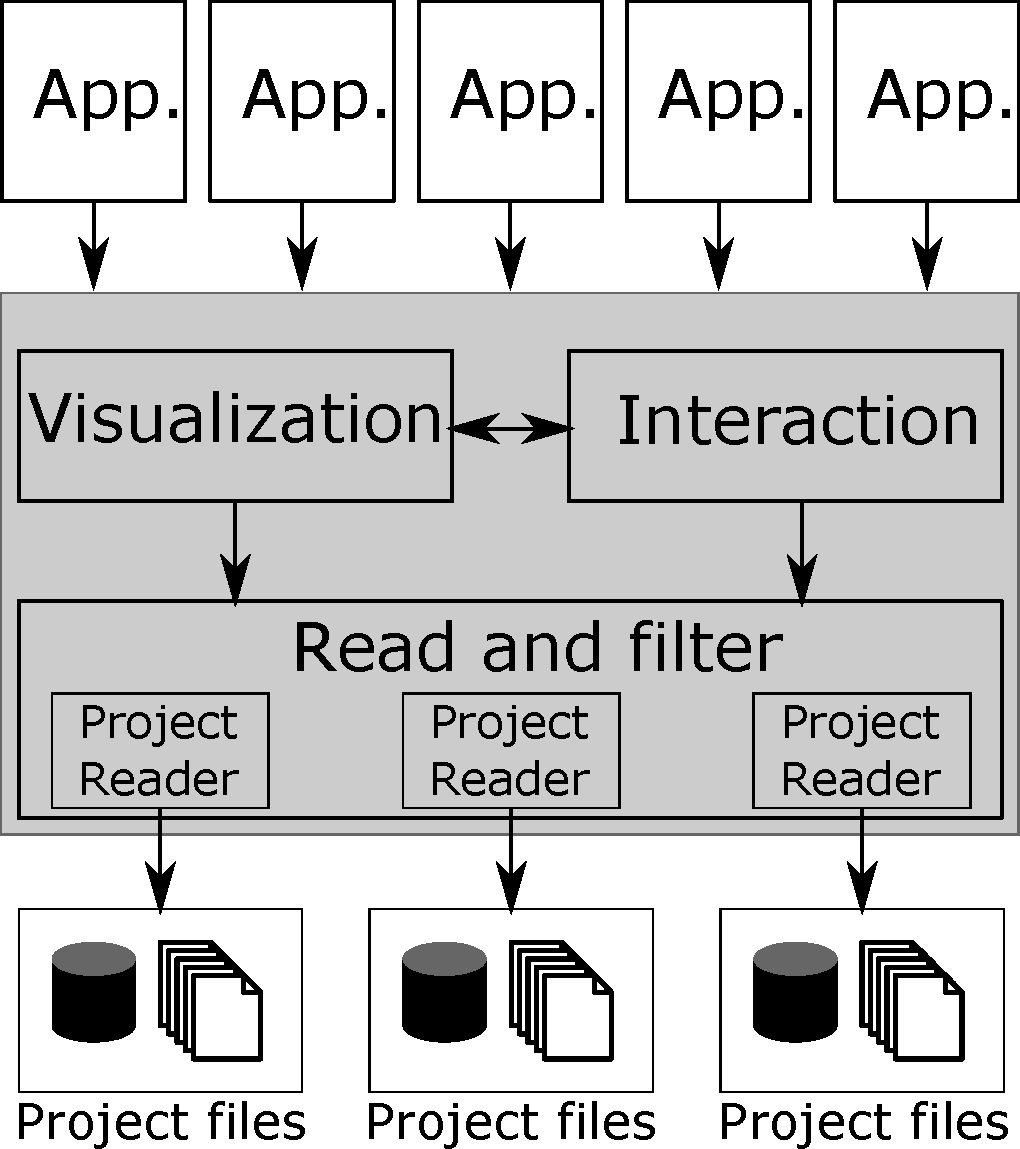
\includegraphics[width=0.6\linewidth]{arquitecture.pdf}
\end{center}
 \caption{\label{fig_arch} The BRAVIZ software architecture}
\end{figure}

\begin{figure}
\begin{center}
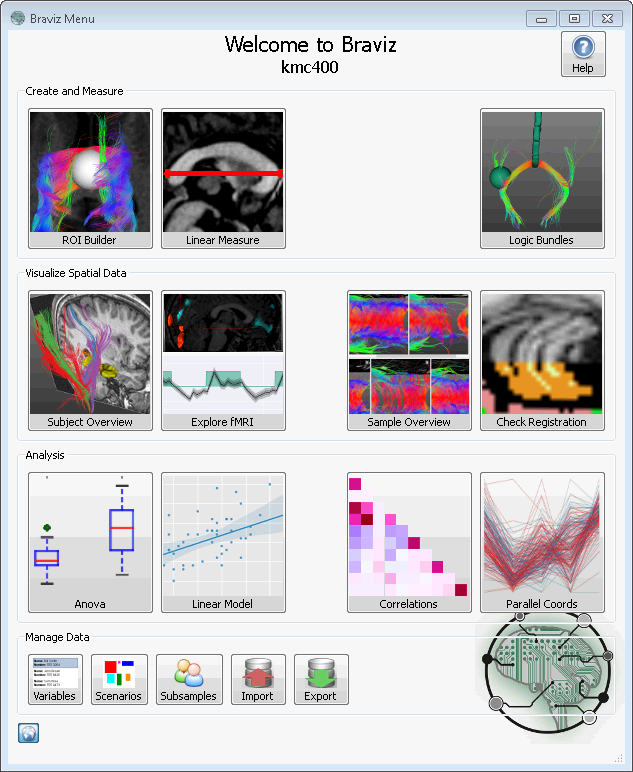
\includegraphics[width=0.4\textwidth]{braviz_menu}
\end{center}
 \caption{\label{fig_menu} BRAVIZ main menu }
\end{figure}

\begin{figure}
\begin{center}
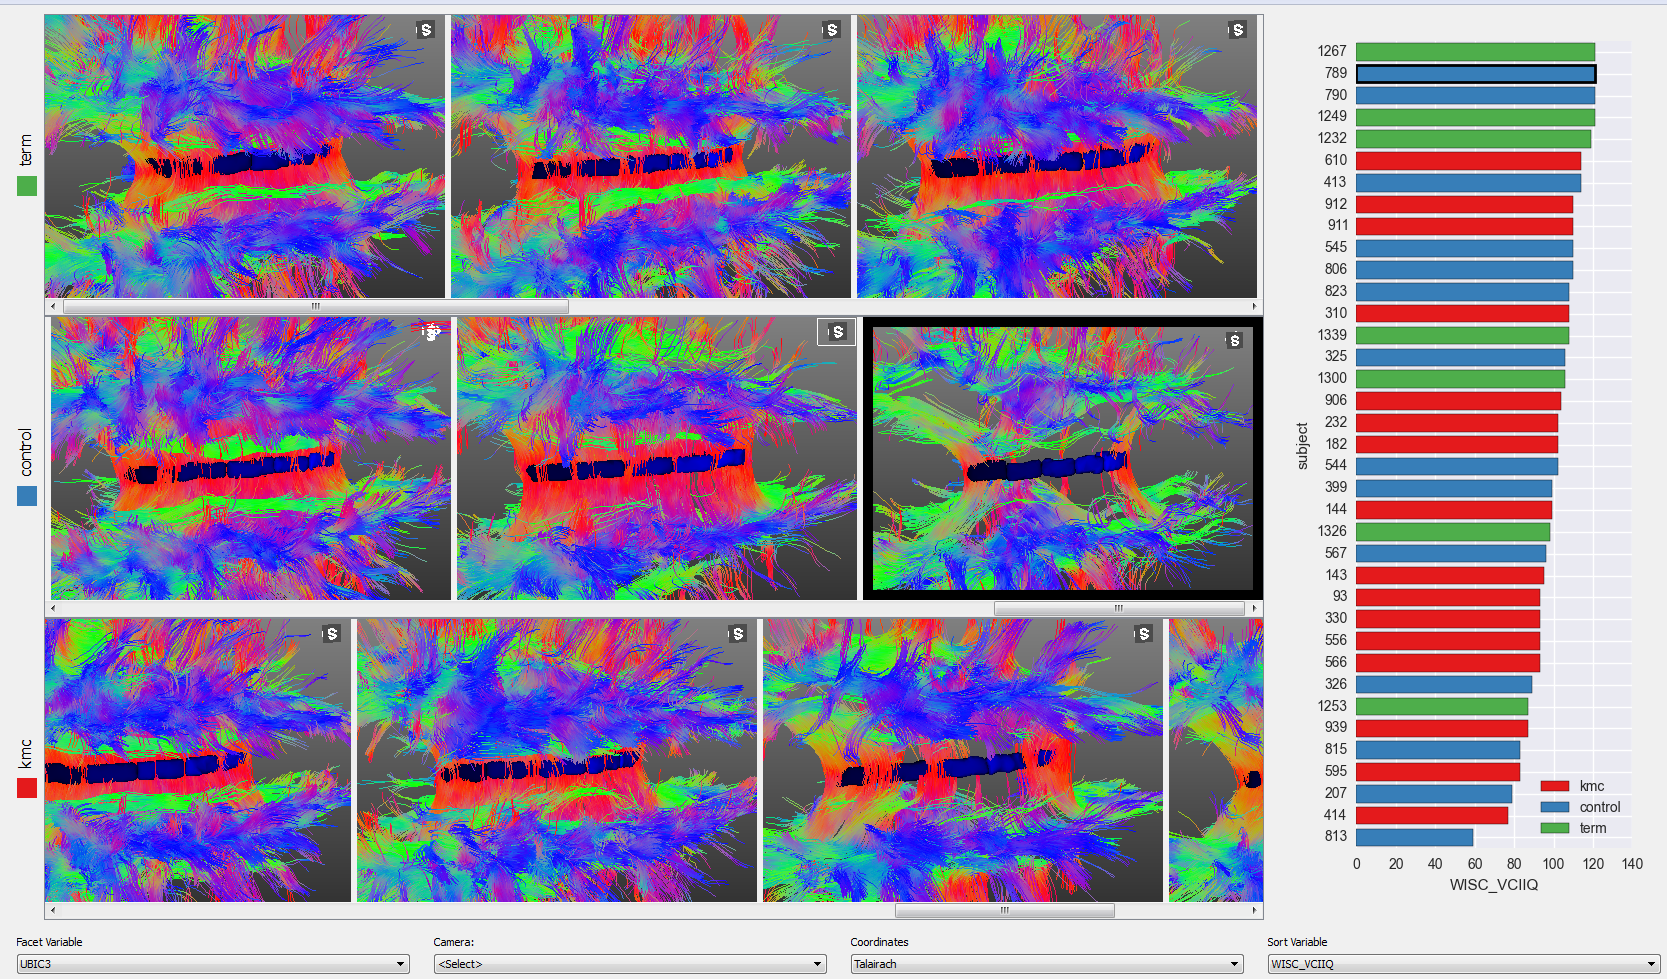
\includegraphics[width=\linewidth]{quality_control_trim}
\end{center}
 \caption{\label{fig_sample} Quality control on the corpus callosum fibers from the whole sample}
\end{figure}


\begin{figure}
\begin{center}
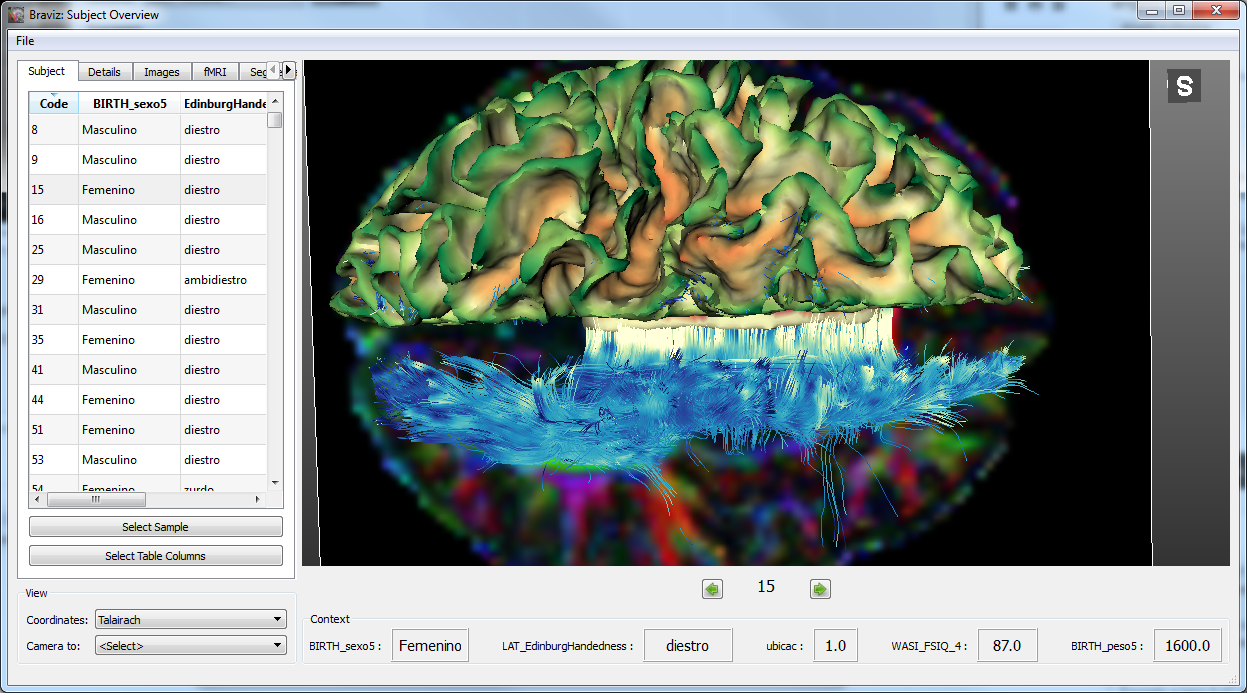
\includegraphics[width=\linewidth]{subj_overview_full}
\end{center}
 \caption{\label{fig_subject}Main interface of the subject overview application: At the bottom of the render some variables about the subject provide context}
\end{figure}

\begin{figure}
\begin{center}
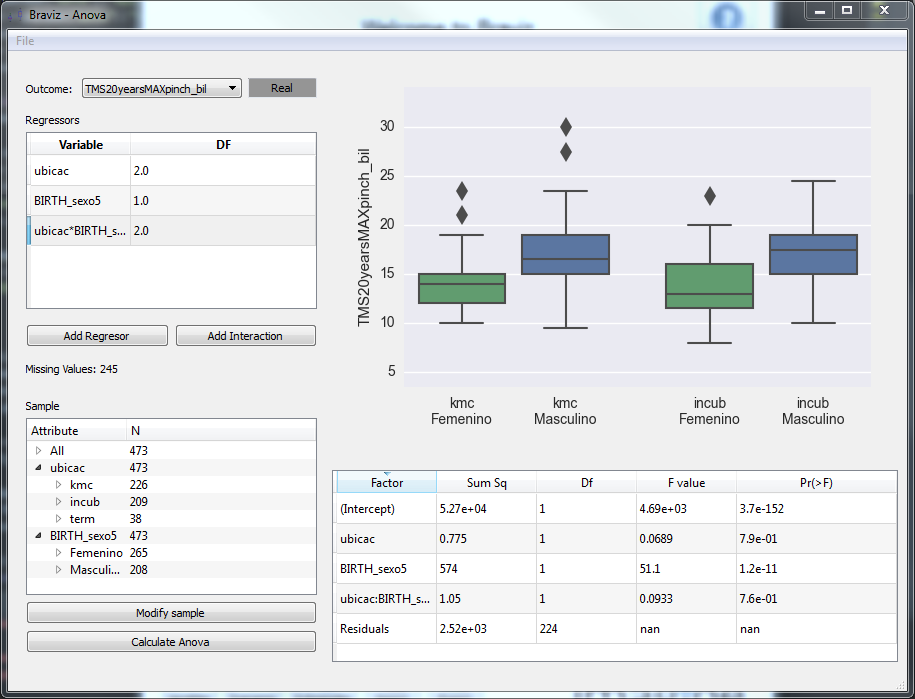
\includegraphics[width=\linewidth]{anova.png}
\end{center}
 \caption{\label{fig_anova}An application for performing ANOVA analyses using the data in the BRAVIZ database.}
\end{figure}

\begin{figure}
\begin{center}
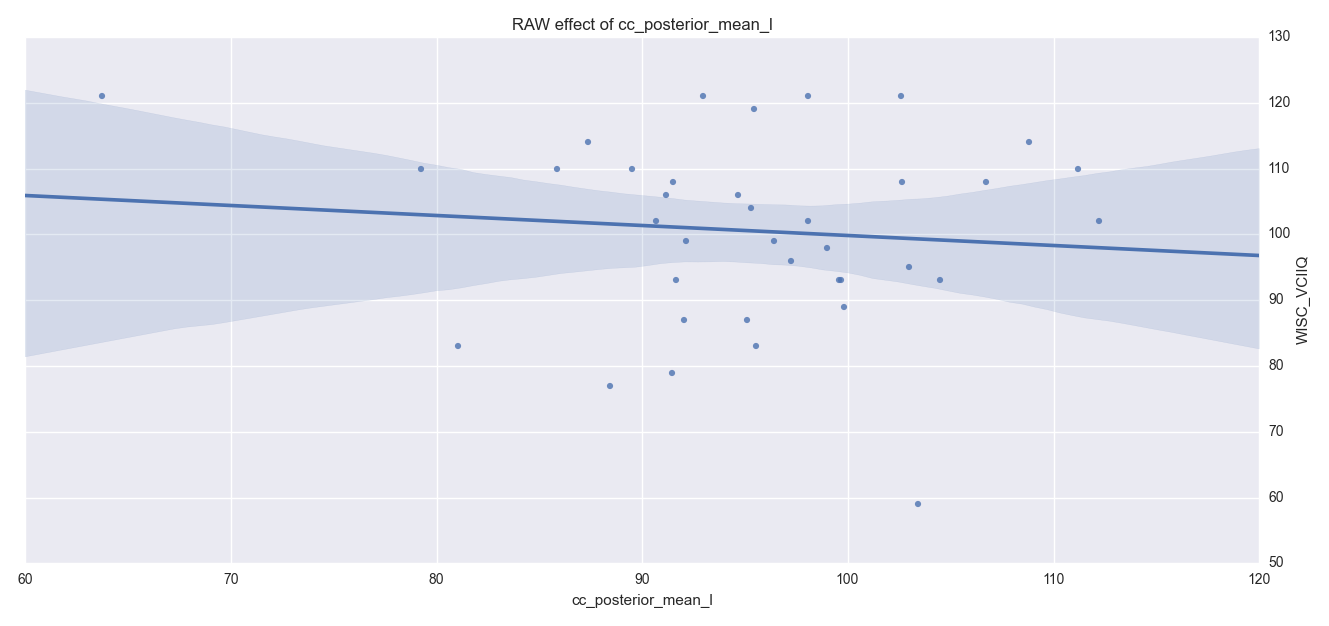
\includegraphics[width=\linewidth]{initial_corr}
\end{center}
 \caption{\label{fig_lm}A correlation with a prominent outlier}
\end{figure}


\begin{figure}
\begin{center}
\begin{subfigure}[b]{0.18\linewidth}
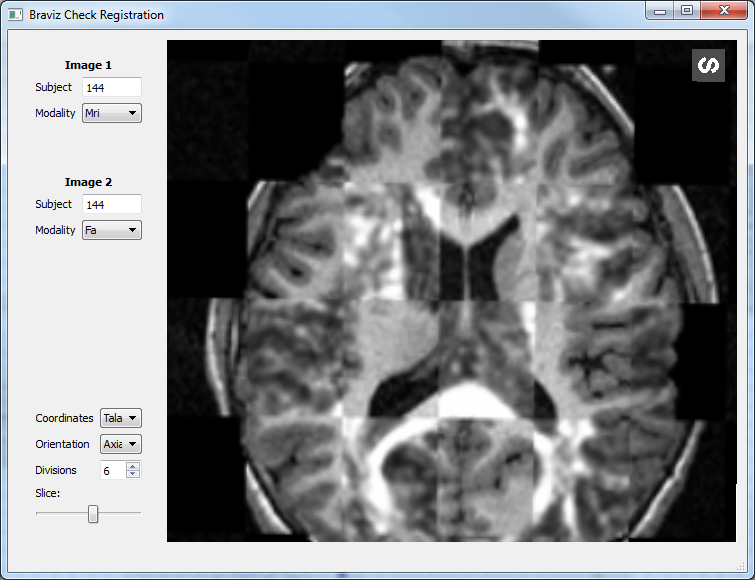
\includegraphics[width=\textwidth]{check_reg}
\caption{\label{fig_check_reg}Check Registration}
\end{subfigure}\hfill
\begin{subfigure}[b]{0.3\linewidth}
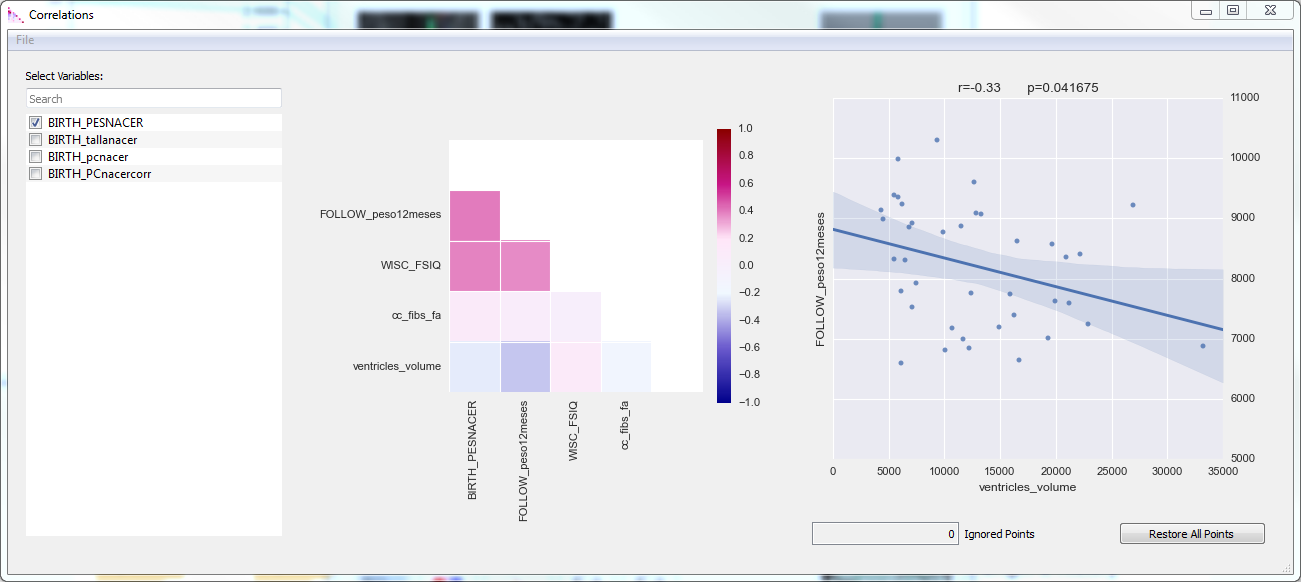
\includegraphics[width=\textwidth]{correlations}
\caption{\label{fig_correlations}Correlations}
\end{subfigure}\hfill
\begin{subfigure}[b]{0.22\linewidth}
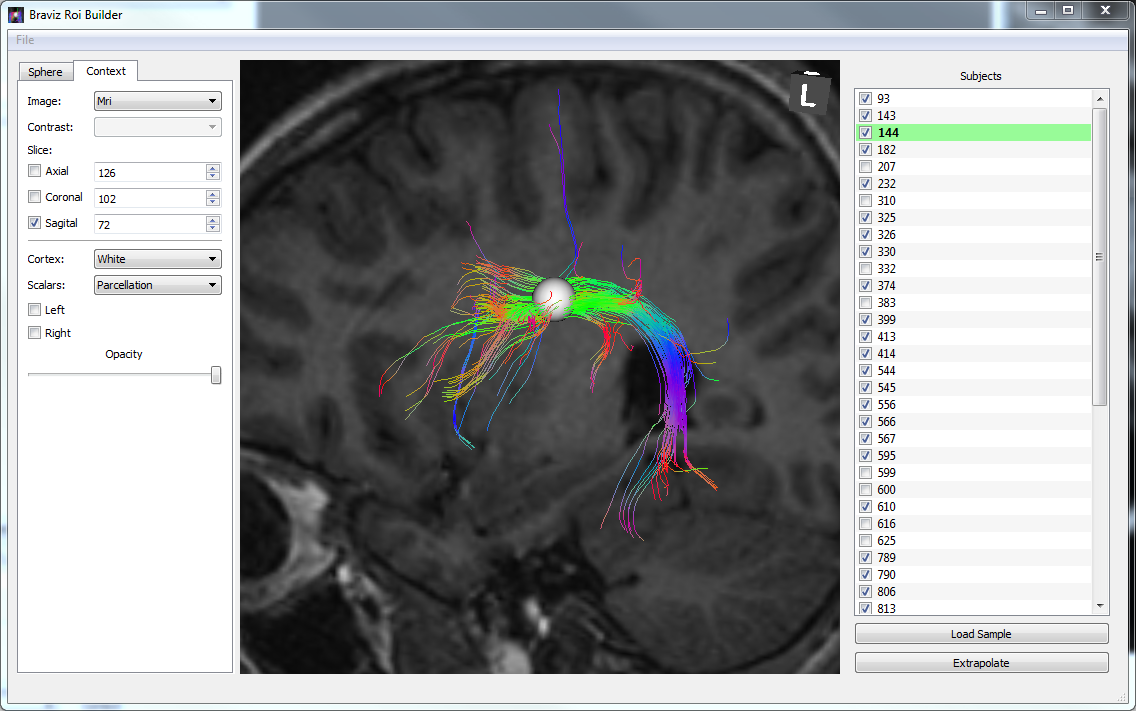
\includegraphics[width=\textwidth]{roi_builder}
\caption{ROI Builder\label{fig_roi}}
\end{subfigure}\hfill
\begin{subfigure}[b]{0.18\linewidth}
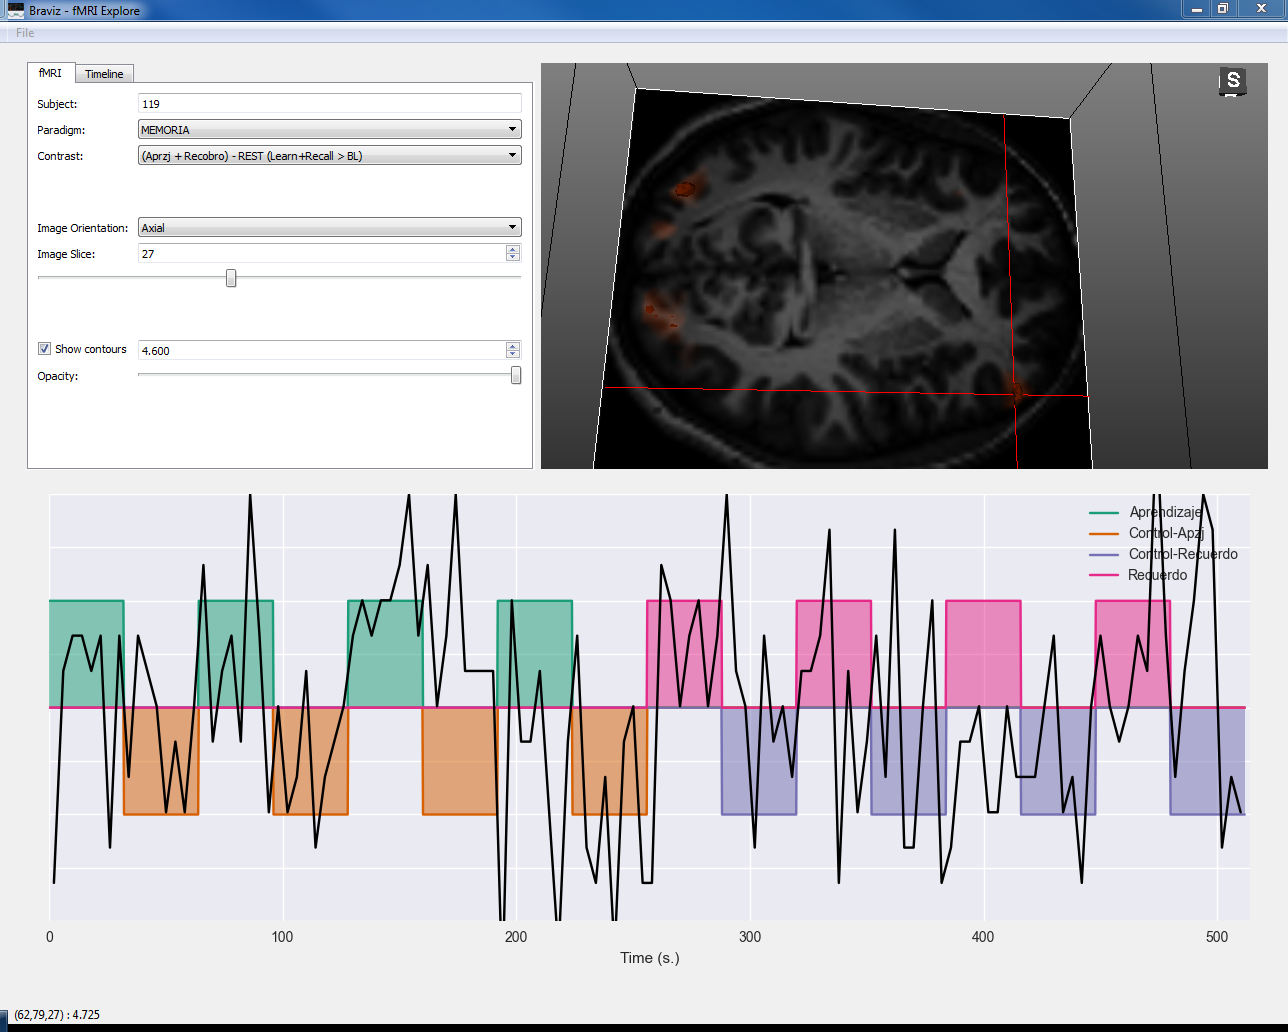
\includegraphics[width=\textwidth]{fmri}
\caption{FMRI Explorer\label{fig_fmri}}
\end{subfigure}
\end{center}
 \caption{\label{fig_other_apps} Examples of BRAVIZ Applications}
\end{figure}

\begin{figure}
\begin{center}
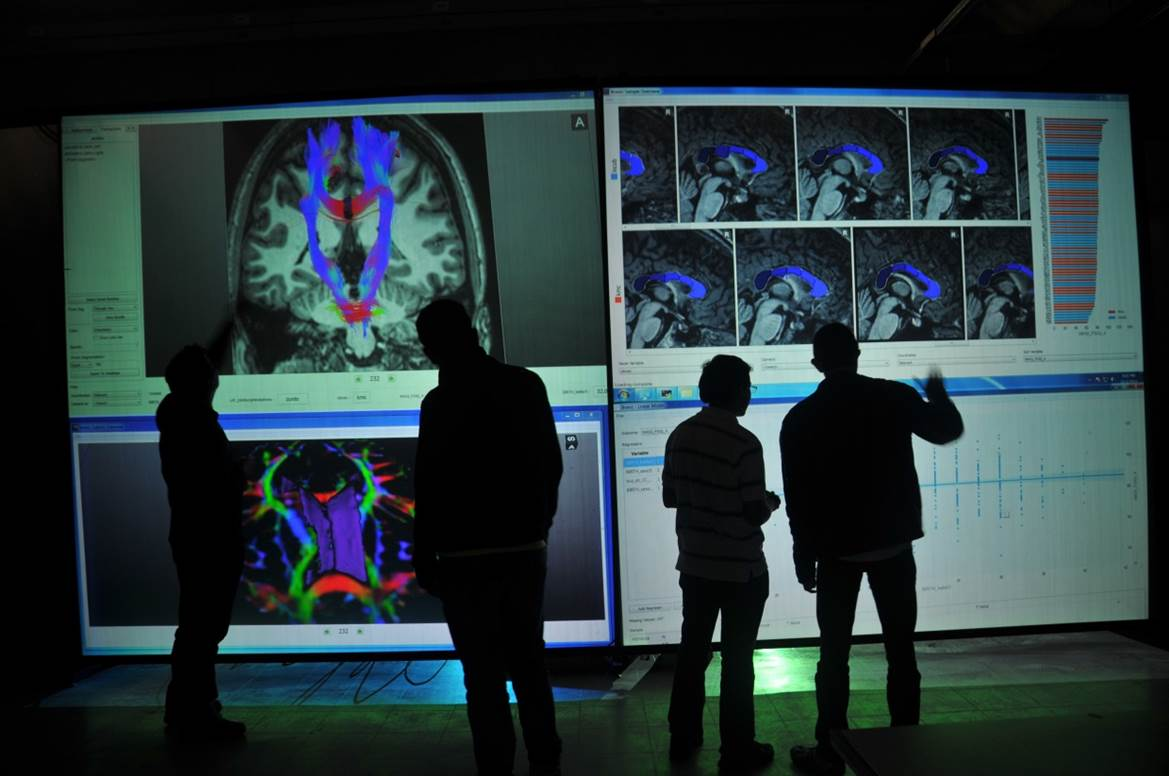
\includegraphics[width=\linewidth]{imagine.jpg}
\end{center}
 \caption{\label{fig_imagine} An example of BRAVIZ running on a large display in a collaborative setting.}
\end{figure}


\begin{figure}
	\centering
		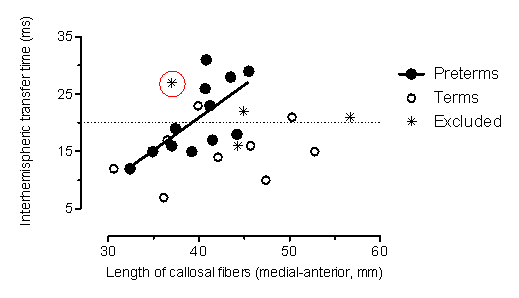
\includegraphics[width=\linewidth]{cyril_plot}
	\caption{Correlation between length of callosal fibers and ITT in the PT and term groups}
	\label{fig_cyril_1}
\end{figure}

\begin{figure}
	\centering
		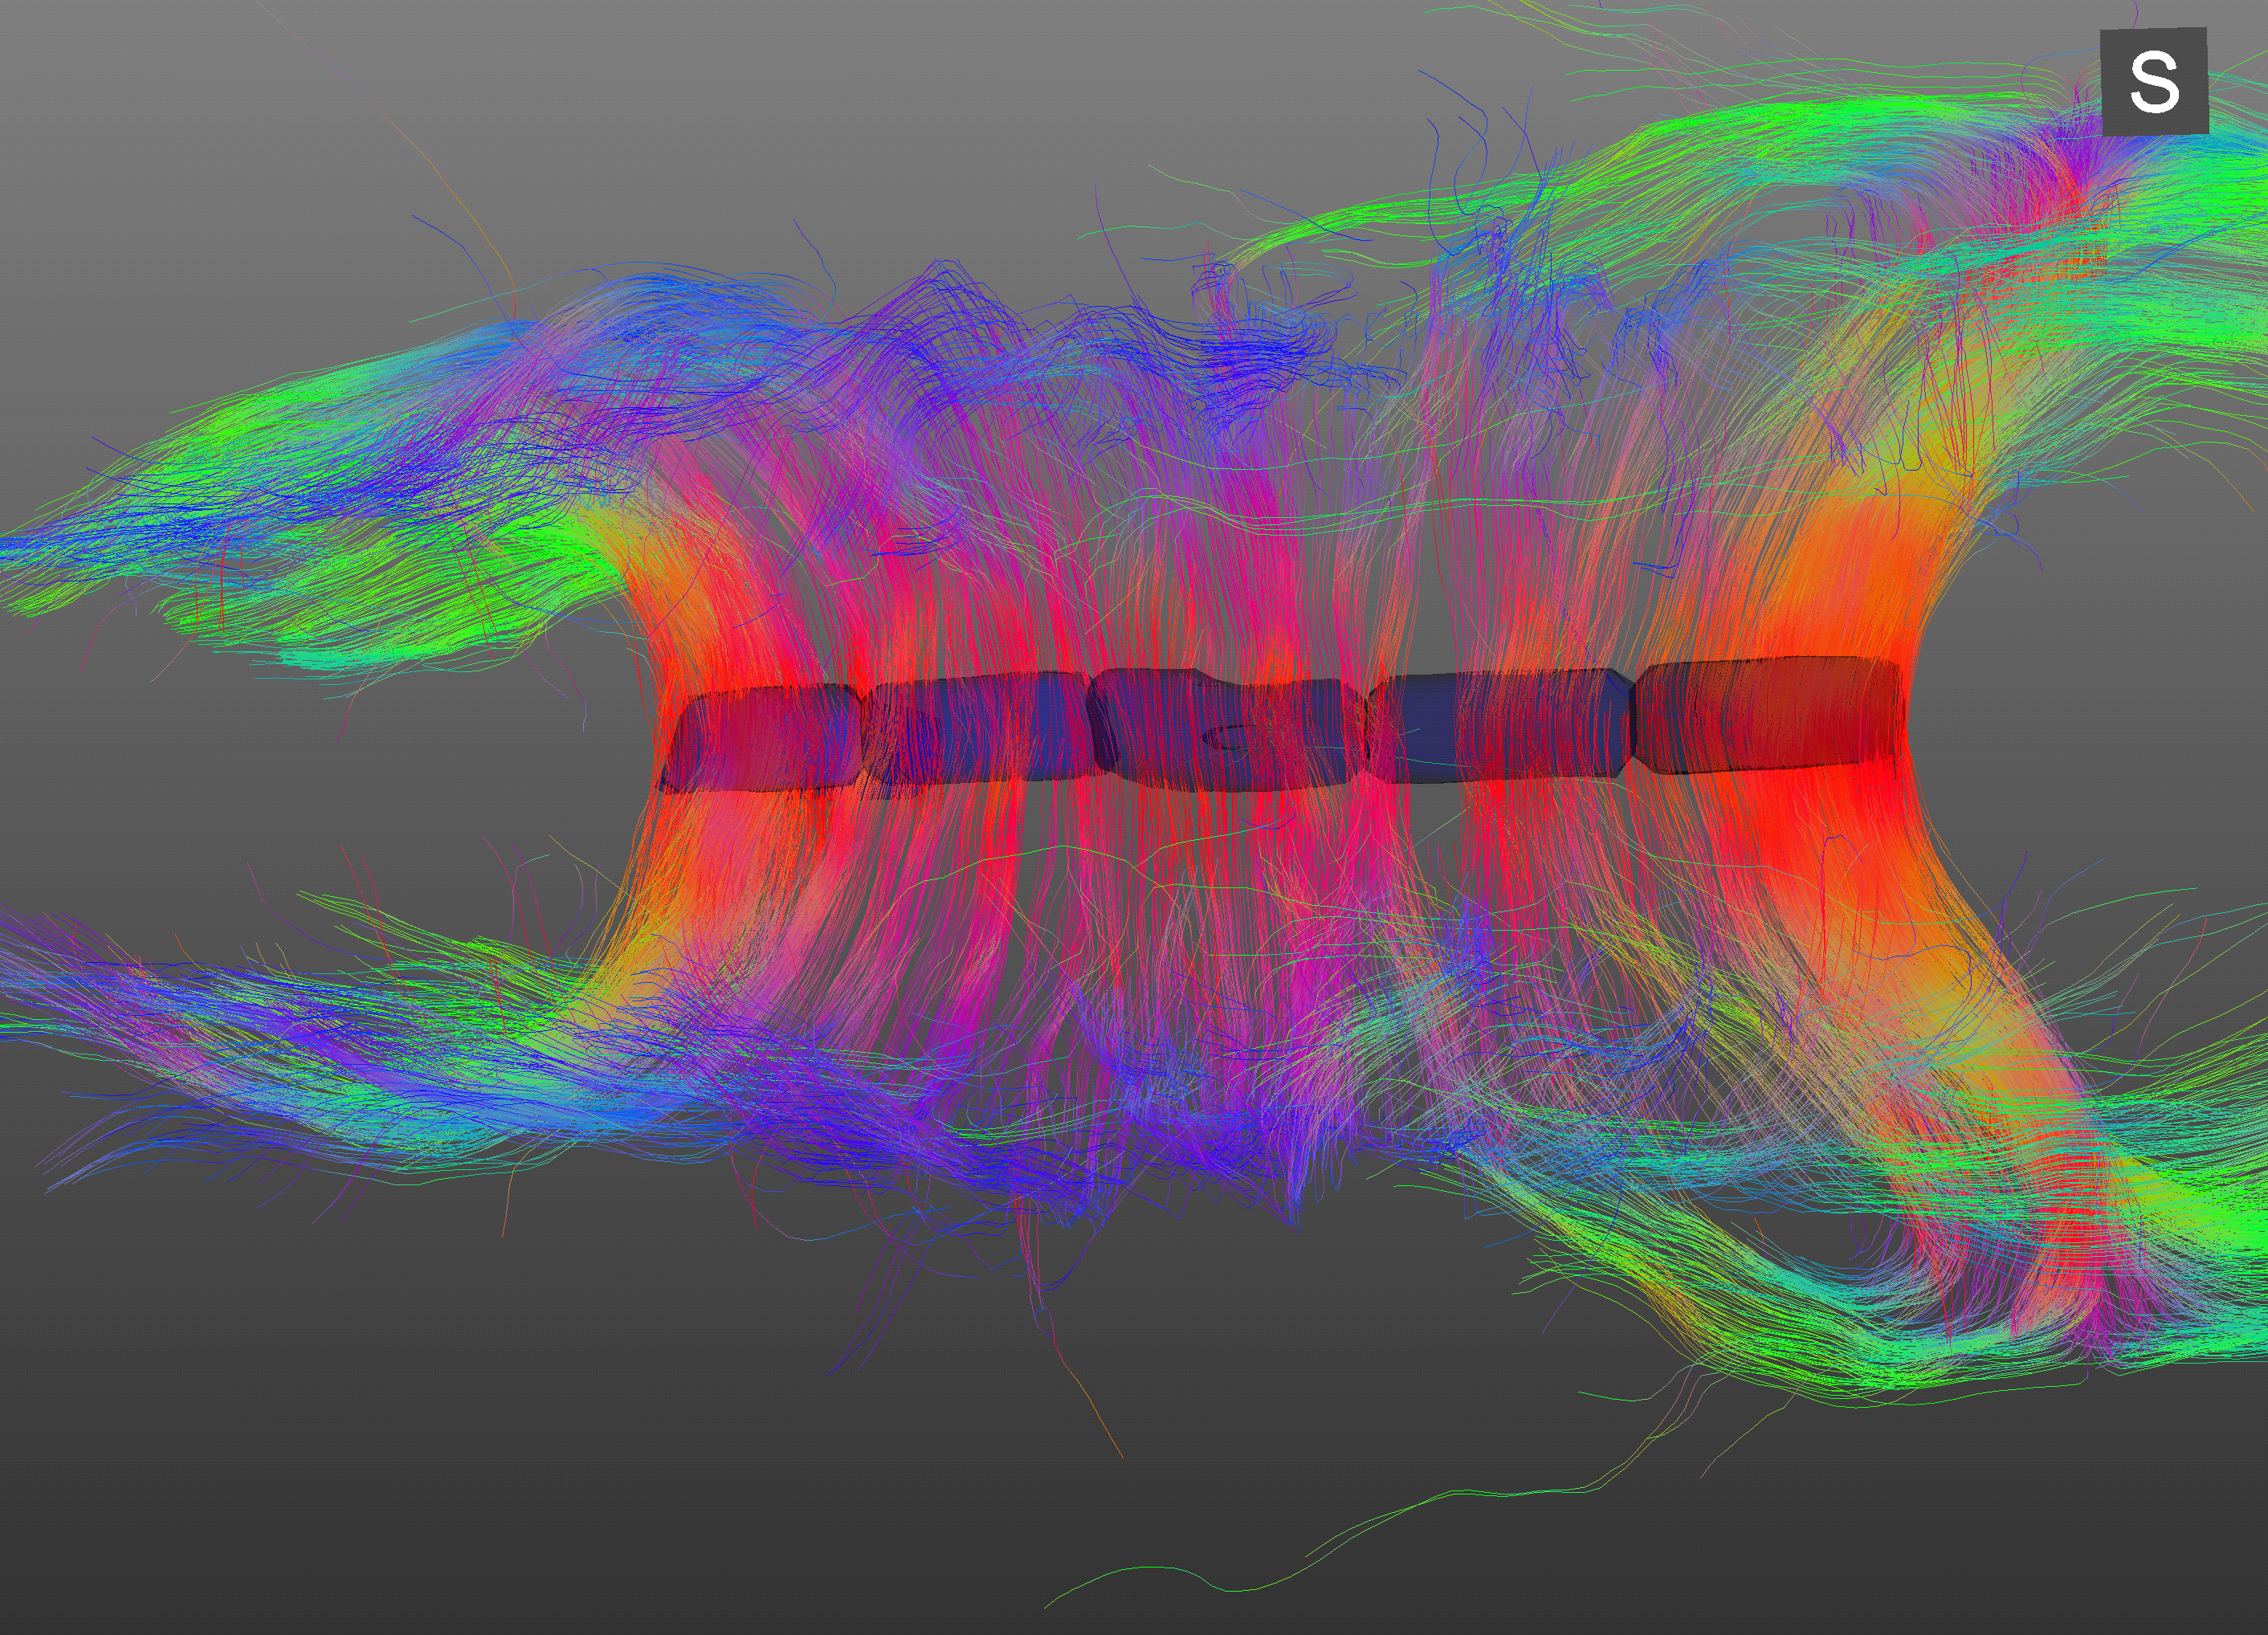
\includegraphics[width=\linewidth]{cc_cyril}
	\caption{Corpus Callosum from the circled outlier in Figure \ref{fig_cyril_1}}
	\label{fig_cyril_2}
\end{figure}


\begin{figure}
	\centering
		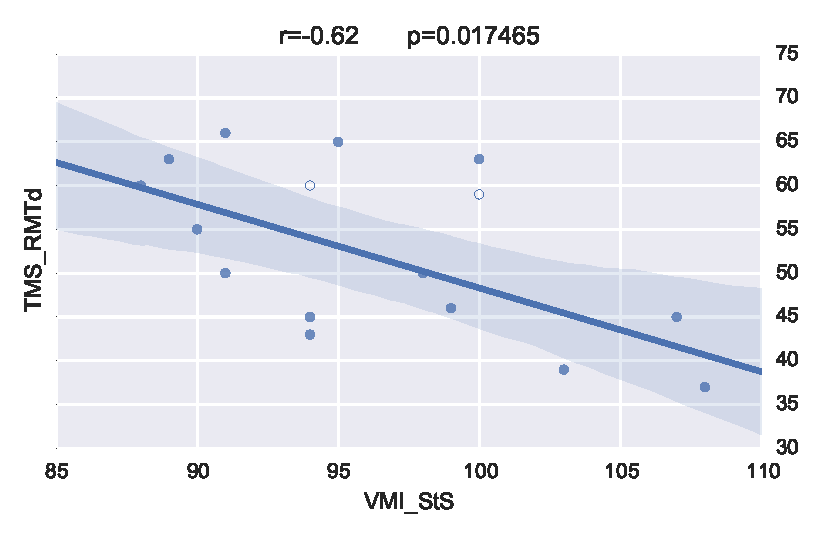
\includegraphics[width=0.9\linewidth]{cyricl_corr_1}
	\caption{VMI vs M1 excitability excluding outliers}
	\label{fig_cyril_4}
\end{figure}

\begin{figure}
	\centering
		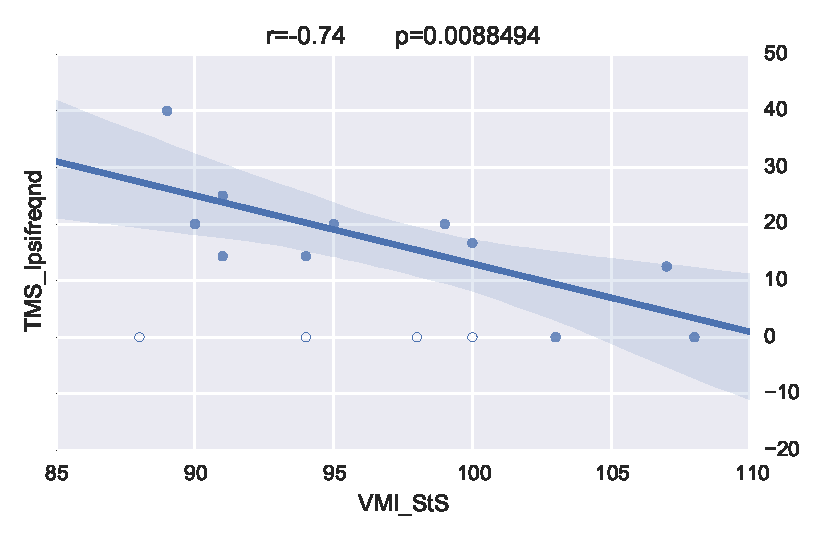
\includegraphics[width=0.9\linewidth]{corr_cyril_2}
	\caption{VMI vs ipsilateral corticospinal responses excluding outliers}
	\label{fig_cyril_5}
\end{figure}

\begin{figure}
\begin{center}
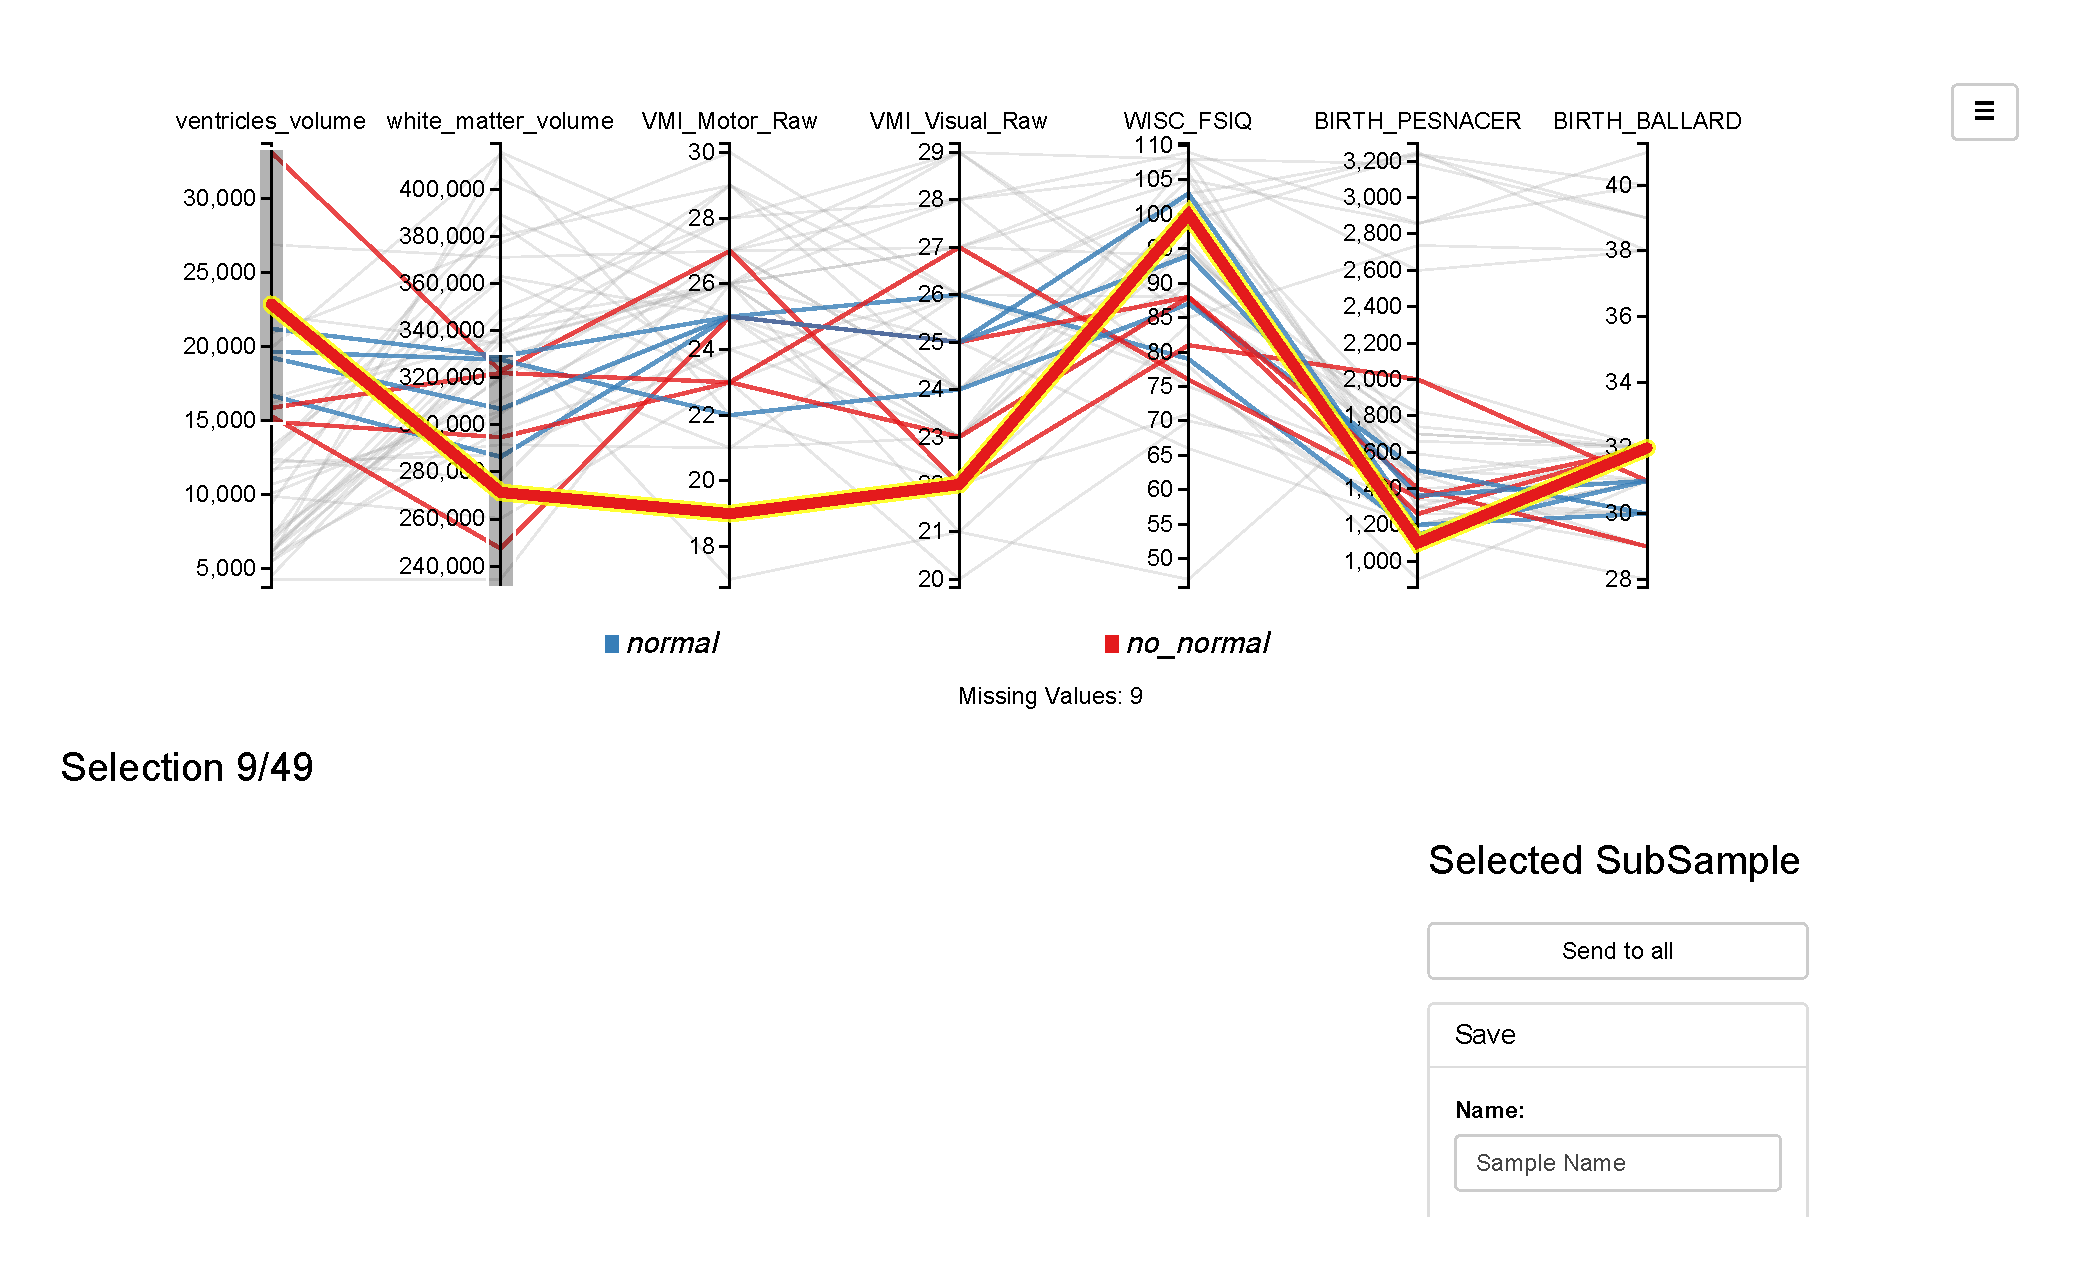
\includegraphics[width=\linewidth,trim = 30mm 90mm 60mm 10mm ,clip]{parallel_coordinates_raw}
\end{center}
 \caption{\label{fig_parallel}Parallel coordinates display configured for searching possible PVL cases}
\end{figure}


\begin{figure}
\begin{center}
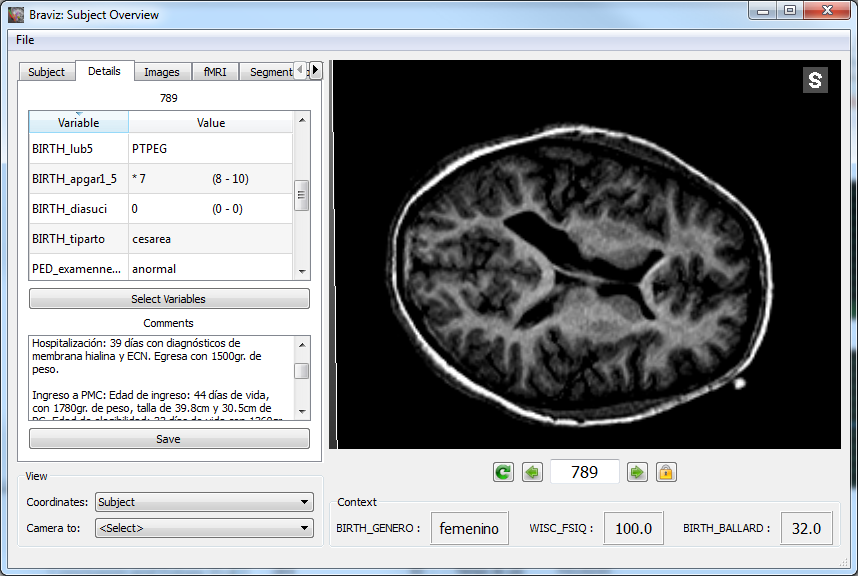
\includegraphics[width=\linewidth]{pvl_details}
\end{center}
 \caption{\label{fig_subject3}Details of a subject with possible PVL, the left panel shows values for several variables as well as the full clinical history.}
\end{figure}

\end{document}
